% ==========================================================================
%	RESEARCH PROPOSAL
% ==========================================================================

% - INTRODUCTION -----------------------------------------------------------
\chapter{Introduction}
\label{ch:intro}
% --------------------------------------------------------------------------

% --------------------------------------------------------------------------
\section{Motivation} \label{sec:intro-motivation}
% --------------------------------------------------------------------------

Cybersecurity has been and still remains \textit{the} most crucial discipline in the domain of \Ac{it}: According to Mordor Intelligence, the global cybersecurity market was valued at approx. \$150 billion in 2021. This trend is expected to continue, rising up to approx. \$317 billion by the year of 2027 with a constant annual growth rate of 13.4\% \cite{noauthor_cybersecurity_2022}. This can be linked to the average cost of a single data breach equaling \$4.24 million in the same year and describing the highest value on record so far, as per IBM \cite{noauthor_cost_2022}. These rises are proportional to the increase in cyber attacks: Malware attacks increased by 358\% in 2020, Ransomeware attacks rose by 435\% \cite{noauthor_malware_2021}.The current landscape of cybersecurity can be summarized as an arms race between the attackers of valuable resources and their protectors. 

Looking at the domain of \ac{cc}, 27\% of organizations report having experienced security incidents within one year \cite{schulze_cloud_2022}. Overall, the fear of security challenges is the main concern why some businesses do not introduce \ac{cc} at all \cite{noauthor_2021_2021, noauthor_2022_2022}.

Businesses investing in sophisticated security technology and services might not be enough, as 95\% of cybersecurity issues can be linked to human error \cite{mee_after_2020}. One reason for this might be the increased complexity of security systems and settings, leading to misconfigurations that in turn lead to security vulnerabilities. In \ac{cc}, misconfiguration in the cloud infrastructure accounted for 23\% of security incidents \cite{schulze_cloud_2022}. It can be assumed that the increased complexity of \ac{it} security features reduces its usability, resulting in a decrease of their efficiency.

The research discipline of \textit{usable security} has recognized this issue and aims at bringing effective \ac{it} security together with information system usability \cite{garfinkel_usable_2014}. Considered separately, there exist several  design and assessment frameworks for security aspects within information systems, e.g., the Security Design Principles by Saltzer and Schröder (1975) \cite{saltzer_protection_1975}, the Security By Design Principles according to the \ac{owasp}, or the Cybersecurity Framework by the \ac{nist} \cite{noauthor_framework_2018}. On the other hand, usability assessments, e.g., the Usability Heuristics by Nielsen (1994) \cite{nielsen_10_1994}, or usability principles and guidelines support the evaluation of the user friendliness of \acp{ui} \cite{moran_usability_2019}. These existing frameworks will hereinafter be referred to as \textit{current frameworks}.

However, usable security research as a whole is considered complicated due to interdisciplinary factors, technological velocity, etc. \cite{garfinkel_usable_2014}. That is why it is currently conducted based on individual definition and execution of experiments rather than supported by guidelines or frameworks. This can lead to slower examination of the problems at hand, consequently leading to fewer insights on how to potentially address them.

This is where this proposed Master's thesis ties in: It suggests a unified framework for qualitative usable security assessment that will be developed and evaluated experimentally within the security-crucial domain of \ac{cc}. This will hereinafter be referred to as the \textit{unified framework}.

% --------------------------------------------------------------------------
\section{Problem Statements} \label{sec:intro-problems}
% --------------------------------------------------------------------------

The previous motivation to the topic (cf. \autoref{sec:intro-motivation}) as well as further demonstration of current research in that area (cf. \autoref{ch:related-work}) recognize the following problems:

\begin{description}
	\item[P1] Usable security research is currently conducted on a case-by-case basis which limits efficiency and quantity of insights in order to address problems within that domain.
	\item[P2] In terms of \ac{cc}, security configuration aspects are currently complicated to consider in terms of usable security, which visibly leads to a significant amount of security incidents.
\end{description}

% --------------------------------------------------------------------------
\section{Contribution} \label{sec:intro-contribution}
% --------------------------------------------------------------------------

The problems stated in \autoref{sec:intro-problems} are aimed at being addressed through the following aspired contributions. While these contributions are build on one another, they are also designed to individually undertake issues within current usable security research.

\begin{description}
	\item[C1] Evaluate the applicability of present usability and security design frameworks to usable security individually to the domain of \ac{cc} in order to deduct limitations and improvements.
\end{description}

This contribution will partly address P1, as there is limited research present regarding the explicit applicability of usability and security design frameworks to usable security. Thus, it cannot be justified that these frameworks are not applicable per se. This contribution's output will generate the input for C2 in order to have a foundation for the design of the unified framework. As this assessment will be pracitically performed within a \ac{cc} environment, this contribution also partly covers P2.

\begin{description}
	\item[C2] Design a unified qualitative usable security assessment framework based on the findings from C1.
\end{description}

This contribution will mainly address P1 by applying the findings from C1 in order to develop a unified framework for usable security evaluation. It is expected that certain aspects of the frameworks under test in C1 will appear in the unified framework, while others might be refined or newly introduced.
	
\begin{description}
	\item[C3] Validate the unified framework regarding improvements in terms of applicability, conclusivity, and efficiency compared to C1.
\end{description}

This contribution, again, addresses P1 and P2 in that the actual benefit of the new framework needs to be validated within a \ac{cc} security feature scope. \\\

All in all, P2 will be addressed across all contributions as each practical application will be done in terms of \ac{cc} security features. The actual methodology for the achievement of the contributions will be outlined in \autoref{ch:approach}.

% --------------------------------------------------------------------------
\section{Proposal Structure} \label{sec:intro-structure}
This \nameref{ch:intro} chapter introduced the motivation to the topic as well as outlined problems and corresponding contributions to the matter. \autoref{ch:foundations} provides necessary background information to the domains of information and cyber security, security design, usability evaluation, usable security research, as well as \acl{cc}. \autoref{ch:related-work} discusses the current research in the area and derives its limitations that are addressed by the contributions of this thesis. \autoref{ch:approach} describes the methodology and process of achieving the aspired contributions. \autoref{ch:organization} outlines the research stakeholders, Master's thesis artefacts as well as the project plan of this work.
% --------------------------------------------------------------------------


% - FOUNDATIONS ------------------------------------------------------------
\chapter{Foundations} \label{ch:foundations}
This chapter aims at providing an overview on the necessary background information and technical foundations required to perform the desired research. It is expected that these foundations will be elaborated in the actual thesis as certain examined aspects of the research might require additional background. The design of this chapter is not meant to be exhaustive to each area but shall only provide the information that is strictly required for the sake of this work.

\section{Information Security} \label{sec:foundations-security}

The U.S. \acf{nist} defines information security as ``the protection of information and information systems from unauthorized access, use, disclosure, disruption, modification, or destruction in order to ensure confidentiality, integrity, and availability`` \cite{nieles_introduction_2017}. The last three characteristics can be further defined:
		
	\begin{description}
		\item[Confidentiality] Unauthorized entities are restricted from access and disclosure of information for the purpose of protecting personal privacy and proprietary information \cite{nieles_introduction_2017}.
		\item[Integrity] Improper modification or destruction of information, including the compromitation of data non-repudiation and authenticity, is protected against. Furthermore, \textit{data integrity} means that data has not been improperly altered, whereas \textit{system integrity} goes beyond unautorized manipulation, defining system function quality when performing as intended and unimpaired \cite{nieles_introduction_2017}.
		\item[Availability] Accessibility and usability of information is reliable and timely \cite{nieles_introduction_2017}. This also includes the prevention of intended, unauthorized withholding of data \cite[p. 36]{fischer-hubner_it-security_2001}.
	\end{description}
		
	This \textit{CIA triad} can be extended by additional characteristics, e.g. \textit{accountability} (user actions can be traced back to them), \textit{functionality} (system's behavior is as intended and expected) and \textit{reliability} (system always performs under equal conditions) \cite[p. 36 sq.]{fischer-hubner_it-security_2001}.
 
\subsection{Distinction from Cyber Security} \label{subs:foundations-security-distinction}

The terms \textit{information security} and \textit{cyber security} (i.a.), are often used interchangeably in literature. However, this work requires a specific distinction between those terms. As defined by the \ac{nist} Cybersecurity Framework, cyber security means ``the ability to protect or defend the use of cyberspace from cyber attacks`` \cite{noauthor_framework_2018}. By that, cyber security is a disciplinary subset of information security that especially considers the electronic protection of data and resources within its technical perimeter. Consequently, this excludes activities like physical access or compliance control that are inherent information security disciplines. Nevertheless, both areas focus on achieving the goal of the information security definition by ensuring the application of the CIA tiad.

\subsection{Security Design} \label{subs:foundations-security-design}
As motivated in \autoref{ch:intro}, cyberattacks are still on the rise, which leads to assume that the current state of the art of security design and implementation cannot systematically exclude security flaws. This has already been recognized by Saltzer and Schröder (1975) who summarized general security design guidelines that address general security problems during the design of information systems \cite{saltzer_protection_1975}. They include best practices that aim at considering the CIA triad from the software perspective.%Their Security Design Principles include the following:

%\begin{description}
%	\item[Economy of mechanism] The design of security measures embodied in both hardware and software should be as simple and small as possible \cite{saltzer_protection_1975}.
%	\item[Fail-safe defaults] Access decisions should be based on permission rather than exclusion \cite{saltzer_protection_1975}.
%	\item[Complete mediation] Every access to resources must be checked against the access control mechanism \cite{saltzer_protection_1975}. In turn, no access should be granted without authorization.
%	\item[Open design] The design of a security mechanism should be open rather than secret \cite{saltzer_protection_1975}. The absence of that rule is also referred to as \textit{security by obscurity}.
%	\item[Separation of privilege] Multiple privilege attributes are required to access a restricted resource \cite{saltzer_protection_1975}.  
%	\item[Least privilege] Every process and every user of the system should operate using the least set of privileges necessary to perform the task \cite{saltzer_protection_1975}.
%	\item[Least common mechanism] Design should minimize the functions shared by different users \cite{saltzer_protection_1975}.
%	\item[Psychological acceptability] Security mechanisms should not interfere unduly with the work of users \cite{saltzer_protection_1975}. Later, it will be shown that this principle laid the foundation for usable security research.
%\end{description}


It appears to support security design aspects during the actual design and implementation. There exist similar design frameworks in that domain, e.g., the \ac{owasp} Security By Design Principles. %They also include aspects of less trust in terms of third-party services as well as the necessity to mitigate security vulnerabilities at their core.

Finally, there exist distinct security assessment and improvement frameworks for information systems that are already in place, such as the \ac{nist} Cybersecurity Framework. It defines a process model for the evaluation of the current state, a tiered readiness assessment, as well as transition profiles to reach a desired state of cybersecurity \cite{noauthor_framework_2018}.%, starting with 

%\begin{itemize}
	%\item the identification of security threats and vulerabilities,
	%\item the development of protection safeguards,
	%\item the detection of security incidents,
	%\item the development of response mechanisms to these incidents, as well as the
	%\item recovery from these events after the fact \cite{noauthor_framework_2018}.
%\end{itemize}

%Furthermore, the \ac{nist} framework also works with a readiness evaluation that assesses the degree of completeness to its security processes. Additionally, the framework defines profiles that support the transition from current, potentially undesirable security measures, to a desired target state \cite{noauthor_framework_2018}.


\section{Usability of Information Systems} \label{sec:foundations-usability}

Information system usability is part of ergonomics of human-system interaction, standardized by the \ac{iso} \cite{noauthor_ergonomics_2020}. It defines \textit{usability} as the ``extent to which a system, product or service can be used by specified users to achieve specified goals with effectiveness, efficiency and satisfaction in a specified context of use`` \cite{noauthor_ergonomics_2020}.

The interaction between the user and the system is done through a \acf{ui}, defined by \ac{iso} as the ``set of all the components of an interactive system that provide information and controls for the user to accomplish specific tasks with the interactive system`` \cite{noauthor_ergonomics_2020}.

While usability design and evaluation are often applied to \acp{ui}, these processes could also apply to less end-user-focussed interfaces, e.g., \acp{api} or \acp{cli}.

\subsection{Usability Design Guidelines} \label{subs:foundations-usability-design}

The process of providing \textit{good} system usability to users is aided by several guidelines and frameworks: The \ac{iso} defines the \ac{hcd} process, which describes an ``approach to systems design and development that aims to make interactive systems more usable by focusing on the use of the system and applying human factors/ergonomics and usability knowledge and techniques`` \cite{noauthor_ergonomics_2019}.

\ac{hcd} is an iterative approach and includes the understanding and requirement of the context, as well as the cooperative development and evaluation of design solutions \cite{noauthor_ergonomics_2019}. The latter steps are aided by potential users of the system under design.

\ac{hcd} is particularized through further guidelines developed by notable researchers that define general principles on usability design. These include, but are not limited to, Shneiderman's Eight Golden Rules of Interface Design \cite{shneiderman_designing_2018}, Norman's Seven Design Principles \cite{norman_design_2013}, and Nielsen's Ten Usability Heuristics for User Interface Design \cite{nielsen_10_1994}. All of those frameworks follow a similar structure in that they specifically ask for the existence or absence of characteristics within the interface, e.g., visibility of things, consistency of design, etc.

\subsection{Usability Evaluation} \label{subs:foundations-usability-evaluation}

The evaluation of usability is often referred to \textit{usability testing} \cite{moran_usability_2019}. Its goals are to identify problems, uncover opportunities as well as learn about the target user's behavior and preferences \cite{moran_usability_2019}. Elements of usability testing include participants (i.e., realistic users of the system), specific tasks or activities performed by the participant, as well as a facilitator (i.e., moderator and creator of the specific activity) \cite{moran_usability_2019}. After performing the activities, the participants are expected to provide feedback to the moderator, whereas the moderator notes insights to the behavior of the participant and the system.

Usability evaluation can be either qualitative (i.e., focussing on distinct insights and findings with regards to user behavior) or quantitative (i.e., focussing on benchmarks, e.g., task success or elapsed time). They are usually conducted in a remote setting, however there also exists in-person usability testing. Finally, it can be performed in a moderated (i.e., interactive) or unmoderated manner (i.e., no interaction between the participant and the facilitator) \cite{moran_usability_2019}.

The definition of tasks for a usability evaluation highly depends on the specific area under test. However, it can be expected that the usability design guidelines (cf. \autoref{subs:foundations-usability-design}) can be taken into account.

\section{Usable Security} \label{sec:foundation-usable_security}

Bringing it all together, \textit{usable security} deals with the design, implementation, and evaluation of the usability of security features and aspects within information systems \cite{reuter_quarter_2022}. Chronologically, it originates from the already mentioned Security Design Principles by Saltzer and Schröder (1975), specifically the final one considering the ``psychological acceptability`` of the mechanisms \cites{reuter_quarter_2022}{saltzer_protection_1975}. Later, Zurko and Simon (1996) novelly suggested to apply usability aspects of software design to security features \cite{zurko_user-centered_1996}. Shortly after, Adams and Sasse (1999) researched usability flaws in terms of password protection from a user perspective and provided recommendations on remedial measures \cite{adams_users_1999}. Since then, the majority of usable security research is focussed on end-user security in terms of password protection and email encryption \cites{reuter_quarter_2022}{whitten_why_1999}. More recently, this field also started to consider developers and \ac{it} professionals as their usability issues in terms of security can lead to severe security vulnerabilities \cite{chiasson_even_2007-1}.

Other than with security \textit{or} usability evaluation, there do not exist established unified frameworks or guidelines for usable security assessment. Some more recent studies suggest certain approaches that will be discussed in \autoref{ch:related-work}. Other than that, usable security is currently performed by means of individual experiments \cite{garfinkel_usable_2014}.

\section{\acl{cc}} \label{sec:foundations-cloud}

The \ac{nist} defines \ac{cc} as ``a model for enabling ubiquitous, convenient, on-demand network access to a shared pool of configurable computing resources (...) that can be rapidly provisioned and released with minimal management effort (...)`` \cite{mell_nist_2011}. It can be seen as the latest form of infrastructure consolidation after the introduction of client-server computing and the rise of datacenter hardware virtualization \cite[p.\ 1]{sehgal_cloud_2018}.
		
In general, \ac{cc} is described by a vendor-consumer relationship, with the vendor being the provider of the \ac{it} resources, and the consumer being the receiver and user of those resources. Depending on the deployment model of the \ac{cc} infrastructure at hand, the vendor can be 
		
\begin{itemize}
	\item internal to an organization or providing isolated resources exclusively to that organization (i.e., \textit{private cloud}),
	\item external, providing resources to multiple entities (i.e., \textit{public cloud}),
	\item or a mix of both \cite{mell_nist_2011}. 
\end{itemize}  
		
The service level defines the level of abstraction of the resources to the consumer and which party is responsible for which layer of application provisioning and deployment. Typically, this includes \ac{iaas} (vendor provides virtualized infrastructure), \ac{paas} (vendor provides virtualized infrastructure as well as the specific operating system, runtime environment, etc. to that platform), and \ac{saas} (vendor provides infrastructure, platform, and specific software deployment) \cite{mell_nist_2011}. 
		
The \ac{nist} laid out several aspects that further define \ac{cc} characteristics, service, and deployment models.
		
\begin{description}
	\item[On-demand self-service] Provisioning of (more) computing, storage, network resources, etc. is done by the consumer without interaction with the \ac{cc} service provider \cite{mell_nist_2011}. This implies a form of automation on the \ac{cc} vendor's end as well as the existence of control and monitoring interfaces for the consumer \cite[p.\ 51]{sehgal_cloud_2018}. 
	\item[Broad network access] The \ac{cc} vendor's services and capabilities are accessible over the network and can be accessed via mechanisms that are already in place for consuming clients \cites{mell_nist_2011}[p.\ 45]{sehgal_cloud_2018}.
	\item[Resource pooling] Resource pooling allows \ac{cc} vendor's to introduce the concept of \textit{multi-tenancy}, where the physical infrastructure that is made available is virtualized and dynamically assigned to distinct consumers, or \textit{tenants}, based on demand or contractual agreements \cites{mell_nist_2011}[p.\ 45]{sehgal_cloud_2018}. 
		In other words, a \textit{pool} of total resources present is made available to multiple consumers based on their \textit{current} needs and re-evaluated over the course of the usage.
	\item[Rapid elasticity] The consumer can dynamically scale their resource capacity up or down as needed. The consumer is not aware of any global resource limitations which make the \ac{cc} resources appear unlimited \cite{mell_nist_2011}.
	\item[Measured service] The consumed services are quantitatively measured by the \ac{cc} vendor for billing, controlling and optimization purposes. This is based on appropriate forms of metering with regard to the service (e.g., number of terabytes of storage consumed within a month). Thus, billing of utilized services is often done on a pay-per-use basis \cite{mell_nist_2011}. Consequently, the more resources are utilized by the vendor, the higher the cost. This process is transparent to both vendor and consumer, allowing for consumption and billing monitoring, control, and reporting \cite{mell_nist_2011}.
\end{description}
% --------------------------------------------------------------------------


% - RELATED WORK -----------------------------------------------------------
\chapter{Related Work}
\label{ch:related-work}

As mentioned in \autoref{sec:foundation-usable_security}, the discipline of usable security has recently gained in importance. Therefore, it is of interest, which aspects of this underlying work are already present in current research, and which aspects of interest have currently not been addressed. The discussion of related work will prove valuable for the identification of current research limitations that need to be addressed by the contributions of this work. As with \autoref{ch:foundations}, it is expected that the consideration of related work might be enlarged during the actual research.

\section{Present Research}

\subsection{General Research on Usable Security}

Starting with a critical look at usable security research, Theofanos (2020) points out that, even though this discipline has been around for a quarter of a decade, there have been little to no achievements to the underlying problem of so-called \textit{security fatigue} observed in user behavior. She points out the major areas where usable security might make a difference (e.g., authentication, encryption, user dialogs, etc.) and appeals to developers and researchers to make this field of study more applicable and practical \cite{theofanos_is_2020}. The arguments and appeals support this proposed work.

More concretely, Acar et al. (2016) recognize the problem of this research field being almost entirely end-user-centric up until now. They suggest specific measures and key research questions in order to consider developers' and \ac{it} professionals' points of view in that domain. This includes the evaluation of interfaces outside of end user scope, introducing secure usability research towards \acp{api}, as well as providing relevant security resources for the development process \cite{acar_you_2016}. Similar claims are made by Green and Smith (2016). They, again, demand more emphasis on secure and usable \acp{api} \cite{green_developers_2016}. These claims support the validity of this work's research topic and will be of great guidance pursuing the goal of developing a qualitative usable security assessment framework.

Chiasson et al. (2007) furthermore propose general design principles to make administrator interfaces more psychologically graspable \cite{chiasson_even_2007}. These were not validated by the authors during research, but can be used as knowledgable input to the design of this work's assessment framework.

Finally, Lennartsson et al. (2020) analyzed current research directions of usable security more thorougly than possible in this work. Apart from other findings, they recognized the urge of ``developing concrete guidelines for implementation of user-centric security`` \cite{lennartsson_exploring_2020}, which, again, validates this work's purpose.

\subsection{Towards Usable Security Frameworks}
Parkin et al. (2010) recognized the psychological distance between technology-driven password policies in contrast to their users and what negative effect this could have on businesses' security. They essentially suggest an \ac{hcd}-driven approach that includes users of the security mechanism and their feedback throughout its entire design phase \cite{parkin_stealth_2010}. However, this approach ties in with how usable security design and evaluation is currently conducted in terms of individual experiments. Plus, the evaluation and enhancement of features potentially in place is missing here.

Similarly, Feth et al. (2017) extended the individual steps of the \ac{hcd} process to include security awareness from the start. They applied their model exemplarily to a smart home use case. Apart from mentioning the models abstractness, they realize their uncertainty regarding the model's applicability to other use case domains \cite{feth_user-centered_2017}. Furthermore, the research appears to combine security and privacy-related aspects. It also leads to assume that it is rather end-user-focussed which ties in with the majority of current usable security research.

This looks differently when considering research performed by Caputo et al. (2016) who manufactured interview questionnaires for different stages of security feature development and introduction (i.e., development, product, and management level). They then performed three case studies validating the applicability of their methodology and falsified some hypotheses from the beginning (e.g., that complicated security measures are \textit{always} more secure, that usability is common sense, and that there \textit{must be} a tradeoff between usability and security) \cite{caputo_barriers_2016}. Although very valuable for further research, the questionnaires provided are very abstract in that their development does not appear to be based on specific domains nor on current usability or security evaluation frameworks. It also puts a large emphasis on management perception as well as benchmarks in the \textit{process} of development and introduction, rather than on the development or evaluation itself.

Conversely, Ambore et al. (2021) present an evaluation approach that is inspired by usability evaluation heuristics. Specifically, they derive heuristics from general usability assessment and refine as well as apply them to the domain of financial technology. They validate their approach by performing usable security assessment in financial organizations and conclude that such evaluation, in fact, improved usable security of the evaluated applications \cite{ambore_development_2021}. This research can be considered as a starting point for the development of this work's unified framework for the different application domain of cloud computing.

Another approach of usable security evaluation is presented by Hausawi and Allen (2015). They introduce a general quantitative evaluation approach in terms of a risk assessment for usable security. The output of the assessment is a numerical value that aims at classifying the overall risk of present or non-present usable security in terms of an application under test \cite{tryfonas_usable-security_2015}. While this approach appears very general and thus applicable to various domains of interest, it might add an additional burden to the process as it is solely quantitative and does not take individual aspects of usable security into account.

\subsection{Research on Cloud Security}
Understanding current security-related \ac{cc} research and its underlying or discovered problems might aid in moving this work's practical approach in a relevant direction.

A variety of researchers claims that the aspects of multi-tenancy \cite{hashizume_analysis_2013, singh_cloud_2017,paxton_cloud_2016,manakattu_security_2020}, extensive virtualization \cite{felsch_how_2015,hashizume_analysis_2013}, and \ac{iam} \cite{almulla_cloud_2010} present the most critical security concerns across \ac{cc} infrastructure management, regardless of their deployment of service models \cite{manakattu_security_2020}. This leads to assume that general features implementing inherent characteristics of \ac{cc} are generally implemented similarly. Consequently, they also share similar security issues.

In slight contrast, Yandong and Yongsheng (2012) mention that public cloud vendors might be more susceptible to cyberattacks as it is known that they store a vast amount of data that could be leveraged for malicious activities \cite{yandong_cloud_2012}. While it can be argued, that many cloud security issues cannot solely be tackled by improving their security feature usability, an understanding of the criticality of those features can support prioritization of validation criteria when designing a unified usable security assessment framework. 

\subsection{Towards Usable Security in the Cloud}
Research on usable security in the domain of \ac{cc} is strongly limited. However, Fahl et al. (2012) propose a way to introduce usable security in terms of \ac{cc} management. They argue that the current way of securing \ac{cc} resources is done via public key infrastructures that are perceived to be very complicated from an end-users point of view. They propose a novel form of user-friendly security mechanism that removes the perceived burden in the form of a distinct security service \cite{fahl_confidentiality_2012}. While it appears valuable that entirely new mechanisms are researched and developed with the primary goal of usability, this research does not consider the improvement of current established systems by enhancing their usability. The reinvention of security mechanisms should be the last resort, as it merely shifts responsibility from one end to another. This, in turn, might lead to entirely new security concerns.

\section{Achievements \& Limitations}

Based on the findings of the evaluation of the related work to that topic, it can be seen that a lot of effort has been put into discussing and partially solving usable security issues. Specifically, the following general research achievements can be summarized:

\begin{description}
	\item[A1] Recognition of the need for more usable security consideration across all human-facing security features, especially outside of end-user applications.
	\item[A2] Following from A1, the specific usable security consideration under the domain of \ac{cc}.
	\item[A3] Recognition of prime security issues within the domain of \ac{cc} outside of the scope of usable security.
	\item[A4] Recognition of more efficient usable security assessment.
	\item[A5] Following from A3, initial development and partial evaluation of such frameworks under limited scope and generalization.
\end{description}	

Following a process of exclusion, the following limitations to that research can be derived:

\begin{description}
	\item[L1] Despite A1, there is currently little effort to focus on developers and \ac{it} professionals in terms of usable security enablement.
	\item[L2] Despite A2 and A3, the efforts in terms of usable security in the domain of \ac{cc} are limited to reinventing security features rather than assessing and improving them from a usable security point of view.
	\item[L3] Despite of A4 and A5, there currently does not exist a unified, qualitative usable security assessment framework that \ac{cc} could benefit from.
\end{description}

With that, the derived limitations can be linked to the problem statements (cf. \autoref{sec:intro-problems}) and proposed contributions (cf. \autoref{sec:intro-contribution}) of this work, which will be done in the following section.

\section{Application of Contributions}
The following relationship of problems, contributions, as well as current research's achievements and limitations shall finally justify the direction and scope of this work:

\begin{itemize}
	\item \textbf{P1} [tedious usable security evaluation] might benefit from addressing\\ \textbf{L3} [lack of unified assessment framework],\\ which will be achieved by sequentially performing\\ \textbf{C1} [applicability evaluation of current frameworks],\\ \textbf{C2} [design of unified framework], and\\\textbf{C3} [validation of unified framework], aided by input given by\\ \textbf{A5} [suggested frameworks from current research].
	\item \textbf{P2} [\ac{cc} security incidents due to misconfiguration] might benefit from addressing\\ \textbf{L2} [lack of usable security assessment of \ac{cc} security features], and inherently\\ \textbf{L1} [little consideration of \ac{it} professionals within usable security research],\\ which will be achieved by the \ac{cc} scope inside\\ \textbf{C1} [see above] and\\ \textbf{C3} [see above], aided by input given by \\\textbf{A2} [initial consideration of \ac{cc} usable security]  and \\\textbf{A3} [prime security challenges within \ac{cc}]. 
\end{itemize}

The specific approach of solving the mentioned problems through the aspired contributions will be outlined in \autoref{ch:approach}.

% --------------------------------------------------------------------------


% - APPROACH ---------------------------------------------------------------
\chapter{Approach}
\label{ch:approach}
% --------------------------------------------------------------------------

This chapter outlines the necessary steps and methodology that is applied in order to achieve the aspired contributions in terms of the desired research goal of this work (\autoref{sec:approach-structure}). This approach definition is not meant to be final and makes no claim to be exhaustive. This is because the practical application of this approach is expected to yield results that either not fit the approach or require extension.

Apart from that, this chapter also identifies underlying assumptions required to perform the work (\autoref{sec:approach-assumptions}) as well as potential risks to the research and their appropriate countermeasures (\autoref{sec:approach-risks})

\section{Research Structure \& Methodology} \label{sec:approach-structure}

In essence, the underlying research methodology will follow an experimental and empirical approach that aims to (i) find limitations and challenges in current frameworks, (ii) develop a unified framework that addresses these issues, and finally (iii) validate its applicability and overall benefit after the fact. The specific measures to be undertaken are outlined in the following.

\subsection{Preparation of Research Environment \& Scope} \label{subs:approach-structure-prepare}

Before pursuing the first contribution of this work, the research environment and scope need to be prepared. Chapters \ref{ch:intro} and \ref{ch:related-work} already established the overall domain under this research will take place, which is \acl{cc}. For that matter, appropriate candidate \ac{cc} offerings and services must be derived in order to have a finite scope of consideration (referred to as $C_{CC_{ofr}}$ and $C_{CC_{svc}}$, respectively). Similarly, this is also the case for the choice of currently used frameworks that solely consider \textit{either} usability \textit{or} security design or evaluation (referred to as $C_{FW_{use}}$ and $C_{FW_{sec}}$, respectively).
Due to limitations in time and scope that come with a Master's thesis, the goal is to have 

\begin{itemize}
	\item three \ac{cc} offerings (denoted as A, B, and C),
	\item five \ac{cc} services (denoted as 1, 2, 3, 4, and 5), as well as
	\item two current usability, and
	\item two current security evaluation or design frameworks.
\end{itemize}

To allow for an independent assessment of the current framework as well as a  controllable validation of the unified framework, the following split is suggested, such that

\begin{itemize}
	\item $A_{CC_{ofr}} \coloneqq \{A,B\} \supset C_{CC_{ofr}}$ defines the assessment set of \ac{cc} offerings,
	\item $A_{CC_{svc}} \coloneqq \{1,2,3\} \supset C_{CC_{svc}}$ defines the assessment set of \ac{cc} services,
	\item $V_{CC_{ofr}} \coloneqq \{B,C\} \supset C_{CC_{ofr}}$ defines the validation set of \ac{cc} offerings,
	\item $V_{CC_{svc}} \coloneqq \{2,3,4,5\} \supset C_{CC_{svc}}$ defines the validation set of \ac{cc} services,
	\item $K_{CC_{ofr}} \coloneqq A_{CC_{ofr}} \cap V_{CC_{ofr}} = \{B\}$ defines the control set of \ac{cc} offerings, and
	\item $K_{CC_{svc}} \coloneqq A_{CC_{svc}} \cap V_{CC_{svc}} = \{2,3\}$ defines the control set of \ac{cc} service. Consequently,
	\item $A_{CC} \coloneqq A_{CC_{ofr}} \times A_{CC_{svc}} = \{A,B\} \times \{1,2,3\} = \{A1,A2,A3,B1,B2,B3\}$ defines the \ac{cc} assessment combination,
	\item $V_{CC} \coloneqq V_{CC_{ofr}} \times V_{CC_{svc}} = \{B,C\} \times \{2,3,4,5\} = \{B2,B3,\dots,C4,C5\}$ defines the \ac{cc} validation combination, and finally
	\item $K_{CC} \coloneqq K_{CC_{ofr}} \times K_{CC_{svc}} = \{B\} \times \{2,3\} = \{B2,B3\}$ defines the \ac{cc} control combination.
\end{itemize}

The total number and setup of the individual candidates is open to discussion and is merely to support the presentation of the upcoming contributions. The concrete candidate choice criteria will be set up during the actual research phase of this work. However, general choice criteria are briefly outlined in the following: 

The choice of offerings will be aided by quantitative indicators (e.g., market share). To allow for comparability, the choice of \ac{cc} services must be done such that each service is similarly implemented and presented across all \ac{cc} offerings. These candidates will then, again, be validated through quantitative indicators (e.g., relevance or popularity).

The choice of current frameworks will solely be done based on its degree of establishment in the corresponding area of application, that is, the most-used design or evaluation frameworks used in either the usability or security domain.

The corresponding \ac{cc} environments will then be set up. These sets of candidates will then serve as the required input for achieving the first contribution C1.

\subsection{C1: Assessment of Current Framework Applicability} \label{subs:approach-structure-assess}
In order to evaluate the applicability of current usability and security design and evaluation frameworks, the candidate sets $C_{FW_{sec}}$ and $C_{FW_{use}}$ will be applied on the \ac{cc} assessment set $A_{CC}$. Specifically, every element of $A_{CC}$ will be individually evaluated by means of all frameworks $C_{FW_{sec}}$ and $C_{FW_{use}}$. This yields the following mapping:

\begin{center}
	$\mathcal{A} \coloneqq A_{CC} \times (C_{FW_{sec}} \cup C_{FW_{use}}) = \{FW_{sec_1}(A1), \dots, FW_{sec_1}(B3), FW_{sec_2}(A1), \dots, FW_{use_1}(A1), \dots, FW_{use_2}(B3)\}$
\end{center}

with $\mathcal{A}$ being the entire set of assessments and its elements being individual assessments mappings of offering service candidates and current frameworks. This yields a total of 24 assessments. Each assessment will be performed manually, noting findings in terms of the usable security applicability for the particular case. It is expected to have the following categories of findings:

\begin{itemize}
	\item pure usability aspects directly related to the application of a usability framework,
	\item pure usability aspects derived from applying a security framework,
	\item pure security aspects directly related to the application of a security framework,
	\item pure security aspects derived from applying a usability framework,
	\item usable security aspects derived from a usability framework, and
	\item usable security aspects derived from a security framework.
\end{itemize}

These categories then yield three applicability degrees:

\begin{enumerate}
	\item aspects that are applicable without change,
	\item aspects that are applicable with change, and
	\item aspects that are not applicable at all.
\end{enumerate}

Furthermore, each assessment is expected to aid the subsequent design process of the unified framework (cf. C2) such that relevant aspects that are missing from the current framework can be derived by justified assumption. After performing each evaluation, the findings and insights can be prioritized in terms of their relevance, how often they appeared, etc.

The results from the control group evaluation will be most thoroughly documented as they will serve as additional input to the validation process of the unified framework (cf. C3).

It is expected that certain cloud services' interfaces do not solely include security aspects, which is why the evaluation will only focus on aspects within the usability that is mostly or entirely security-related.

The ultimate design of this proposed assessment will be revised after deciding on the specific \ac{cc} offerings, services, as well as current frameworks, if necessary. In any case, the output of the total assessment will be subsequently used in the next contribution C2.

\subsection{C2: Design of Unified Qualitative Usable Security Assessment Framework} \label{subs:approach-structure-design}

The findings from C1 are now applied in order to design the unified qualitative usable security assessment framework, as part of the second contribution.

The design will consider the following findings in order:

\begin{enumerate}
	\item High-priority aspects from current frameworks that can be taken over without change.
	\item High-priority aspects from current frameworks that can be taken over with change.
	\item Low-priority aspects from current frameworks that can be taken over without change.
	\item Low-priority aspects from current frameworks that can be taken over with change.
	\item High-priority aspects derived by justified assumption.
	\item Low-priority aspects derived by justified assumption.
\end{enumerate}

After each step, it is validated that the included steps are not redundant to the previously undertaken step. Finally, after performing all steps based on all findings from C1, all aspects are considered in total in terms of consolidation or generalization, if applicable.

Again, the ultimate design of this proposed framework development process will be revised after having the actual assessment of the current frameworks. In any case, this contribution is expected to yield a unified framework that is similar to the mode of application to the previously chosen, current frameworks. This framework is now subject to validation in terms of the third and last contribution C3, outlined in its separate \autoref{ch:evaluation}.

\section{Assumptions \& Limitations} \label{sec:approach-assumptions}
As certain limitations might not be clear until the start of the actual Master's thesis development, this list of assumptions and limitations makes no claim to be exhaustive.

\begin{description}
	\item[Lack of Budget] At the time of creating this research proposal, it is expected that the research to-be-conducted will not receive any financial support which might be beneficial to the evaluation of paid services or offerings. This limits the choice of \ac{cc} offerings and services to free-tier availability. 
	\item[Positioning of \acs{hpe}] This research is conducted in cooperation with the author's employer and requires that their \ac{cc} offering is taken into account. Therefore, one of the supposedly three \ac{cc} offerings must be covered by \textit{\acs{hpe} GreenLake}. 
	\item[Operational Correctness \& Integrity] As this research does not aim at revealing operational issues of the chosen \ac{cc} offerings or services, it is expected that the deployments perform as intended by the provider.
	\item[Agnostic Implementation] In order to allow for general applicability across \ac{cc} offerings, this research does not differentiate between \ac{cc} deployment models for the assessment, development, and validation of the framework(s). Thus, it assumes that the implementation of service configuration interfaces as well as of underlying security features is generally similar.
	\item[Framework Design] The choice of current frameworks is limited to heuristics, guidelines, or principles that do not explicitly define the approach on how they are applied. The goal is to create a unified framework that can be applied on various application approaches and settings (e.g., both moderated \textit{and} unmoderated). This leads to the research not being validated by actual users as the design of application scenarios of the unified framework lies outside the scope of this work.
\end{description}

Overall, further limitations to the scope and complexity of this proposed research are expected as for the given nature of Master's thesis, that is, a limited working time frame of six months, a generally limited amount of content pages (approx. 60-80 pages), and the fact that the work is conducted in a cooperative study manner next to a full-time employment as given by the study program of the HECTOR School.

\section{Risk to the Research \& Mitigation} \label{sec:approach-risks}

As certain risks to this proposed work might not be clear until the start of the actual Master's thesis development, this list of risks and risk mitigations makes no claim to be exhaustive. It does also not contain superior risks outside of the scope of the research and outside the control of the stakeholders (e.g., sickness, emergency situations, etc.). 

\begin{description}
	\item[Misrepresentation of Research Novelty] The analysis of the related work (cf. \autoref{ch:related-work}) has been and will be done to the best of the author's knowledge and belief, especially in terms of describing the present research's limitations. However, it is possible that relevant work is disregarded (e.g., due to unavailability, etc.) that might render this research's contributions less novel than they were expected. In that case, this will be remedied through scope readjustment.
	\item[Misinterpretation of Complexity] During the practical application of the research approach (cf. \autoref{sec:approach-structure}), it is possible that intermediate results yield (i.a.) the unexpected applicability of current frameworks in terms usable security, or, in contrast, their absolute inapplicability, which could distort the expected value of this research. Again, this will be remedied by means of research scope readjustment.
\end{description}

% - EVALUATION -------------------------------------------------------------
\chapter{Evaluation (C3)}
\label{ch:evaluation}
% --------------------------------------------------------------------------

The validation of the unified framework is expected to assess its validity and benefits compared to current frameworks as well as overall evaluate the success of this research. It also defines the final contribution C3 of this work. This will be done in two steps; (i) the validation by means of the control set $K_{CC}$ as well as by means of the remaining feature set $V_{CC}$.

As the control set features have already been assessed by means of the current frameworks, this form of validation can evaluate efficiency, conclusivity, and applicability in comparison to those frameworks. Since these features have been used to design the framework, there is the risk that it is rather tailored to the particular feature set rather than generally applicable (i.e., \textit{overfitting}). For that, the remaining validation set is used. Even though it cannot compare its outcome with current frameworks, it can validate if the unified framework is generally applicable, efficient and conclusive outside of its design space (i.e., specific cloud offerings \textit{and} services. In short:

\begin{description}
	\item[Comparison of Operation] $\mathcal{K}_c \coloneqq K_{CC} \times (C_{FW_{sec}} \cup C_{FW_{use}}) = \{FW_{sec_1}(B2), \dots, FW_{use_2}(B3)\}$ compared with $\mathcal{K}_u \coloneqq K_{CC} \times FW_u = \{FW_u(B2), FW_u(B3)\}$
	\item[Validation of General Applicability] $\mathcal{V} \coloneqq (V_{CC} \setminus K_{CC}) \times FW_u = \{FW_u(B4), FW_u(B5), FW_u(C2),\\ FW_u(C3), FW_u(C4), FW_u(C5)\}$,
\end{description}

with $\mathcal{K}_c$ being the control set assessment of current frameworks, $\mathcal{K}_u$ being the control set assessment of the unified framework, and $FW_u$ being the unified framework application. 

Again, as with previous contributions, the ultimate design of this proposed evaluation process will be revised after having the actual framework design in place. This is because the nature of a qualitative framework complicates performing a quantifiable evaluation. In any case, this evaluation will conclude the work by answering whether this unified framework actually solves (or, at least, partially addresses) the underlying problems of this thesis (i.e., slow case-by-case approach for usable security research as well as little consideration of non-end-users), critically consider shortcomings of the developed framework, and finally suggest further research in that particular area.

% - ORGANIZATION -----------------------------------------------------------
\chapter{Organization}
\label{ch:organization}
% --------------------------------------------------------------------------

	\section{Research Stakeholders} \label{sec:organization-stakeholders}
	
	The Master's thesis will be conducted by \textbf{Oliver Rudzinski} (oliver.rudzinski@hpe.com).
	\begin{description}
		\item[KIT affiliation] M.Sc. Candidate for Information Systems Engineering and Management at the HECTOR School of Engineering and Management (Technology Business School of the KIT)
		\item[\acsu{hpe} affiliation] Infrastructure Technology Architect for the \textit{Value Solutions} department at the \acl{hpe} Sales Center GmbH in Berlin, Germany. 
	\end{description}
	
	The following stakeholders affiliated with the Karlsruhe Institute of Technology are identified.
		
	\begin{description}
		\item[Reviewer] Prof. Dr. Ralf Reussner (ralf.reussner@kit.edu)
		\item[Second Reviewer] Dr. Robert Heinrich (robert.heinrich@kit.edu)
	\end{description}
	
	Additionally, as the Master's thesis will be conducted in cooperation with the author's employer, the following stakeholder(s) affiliated with \ac{hpe} are identified.
	
	\begin{description}
		\item[Manager] Markus Leitzgen | Inside Sales Manager \textit{Value Solutions} (markus.leitzgen@hpe.com) 
	\end{description}
	
	It shall be noted that additional subject-matter experts, closely related to the \ac{hpe} GreenLake business unit, might be brought in for supporting purposes, or out of interest to their business.	

% --------------------------------------------------------------------------

	\section{Artefacts} \label{sec:organization-deliverables}
	This section outlines the artefacts that are expected to be developed during the process of the Master's thesis. This research proposal document serves as the first artefact. The Master's thesis documentation itself will contain the following artefacts:
	
	\begin{itemize}
		\item description of foundational background to this work (as prepared in \autoref{ch:foundations})
		\item analysis and discussion of related work in the underlying research area (as prepared in \autoref{ch:related-work})
		\item definition of research scope by means of \ac{cc} offerings, services, usability, and security frameworks as well as their classification into assessment, control, and validation sets (as described in \autoref{subs:approach-structure-prepare})
		\item quantified assessment documentation of current frameworks (coinciding with C1, as described in \autoref{subs:approach-structure-design})
		\item unified framework definition (coinciding with C2, as described in \autoref{subs:approach-structure-design})
		\item evaluation of framework and total research approach (coinciding with C3, as described in \autoref{ch:evaluation})
	\end{itemize}
	
	The preliminary versions of these artefacts will be summarized in a presentation that will be held during the thesis' colloquium 4-6 weeks prior to submission. The corresponding presentation slides serve as another artefact to this research.
	
	In case any source code or configuration files are created during the evaluation process of this research, they will be included in adequate manner.
	
	Furthermore, it is expected that the findings of this research will also be presented to an interested audience at \ac{hpe}, which lies outside of the scope of the formal valuation of the thesis.

% --------------------------------------------------------------------------

	\section{Work Schedule} \label{sec:organization-schedule}
	According to the Master's thesis information sheet issued by the HECTOR School, the extent of the Master's thesis for the study program \textit{Information Systems Engineering and Management} is described by 20 ECTS points that correspond to a workload of 600 hours and a development time frame of six months. At the time of this proposal, the official starting date is not yet confirmed. In any case, for the first five months of the thesis development, a rough work capacity of 25 hours per week is expected, which will be increased to 50 hours per week in the last month, excluding the time frames of the remaining HECTOR school modules. This is taken into account for the specific planning of the milestones.
	
	The desired starting date of the thesis development corresponds to the \textbf{1\textsuperscript{st} of October 2022}, which yields the submission date of the \textbf{31\textsuperscript{st} of March 2023}.
	
	It is highly desired to have regular update and mentoring sessions with the reviewers and remaining stakeholders of this research.
	
	\subsection{Work Packages}
	The work packages of this research roughly coincide with the proposed research approach (cf. \autoref{ch:approach}) and evaluation (cf. \autoref{ch:evaluation}).
	
	The preparation work phase (phase 1, cf. \autoref{subs:approach-structure-prepare}) aims at developing criteria for choosing appropriate \ac{cc} offerings and services, followed by deciding on the corresponding elements for this research. Subsequently, this is also done to current security and usability assessment frameworks. Finally, the assessment, validation, and control sets are defined as well as the corresponding \ac{cc} environments prepared. Phase 1 is overlapped by the permanent documentation phase in that the preparatory work is documented as well as the \nameref{ch:foundations} chapter refined.
	
	Phase 1 flows into the assessment phase of current frameworks (phase 2, cf. \autoref{subs:approach-structure-assess}). Before starting with the actual assessment, its proposed approach is refined as well as relevant assessment KPIs defined. Then, the assessments are performed. Findings are derived in parallel to the assessments, and finalized by means of a total assessment insight priorization. As before, the documentation phase overlaps in that the entire process is documented. \nameref{ch:related-work} refinement is also done in that phase.
	
	Phase 2 then flows into the design phase of the unified framework (phase 3, cf. \autoref{subs:approach-structure-design}) with the evaluation of the total findings from phase 2. With that, the framework design approach can be refined, if necessary, that is subsequently used for the actual development of the unified framework. Upon finalizing the framework, it is thoroughly examined in terms of redundancy, possibility of abstraction, etc. Again, the documentation phase runs in parallel by documenting the design approach refinement as well as the actual process of framework development. Further potential \nameref{ch:foundations} and \nameref{ch:related-work} refinement is also done in that phase.
	
	Phase 3 flows into the last practical work phase of evaluating the new framework as well as the entire approach (phase 4, cf. \autoref{ch:evaluation}). This, again, starts with a potential refinement of the evaluation strategy, followed by the comparative evaluation by means of the control set as well as the validation of general applicability via the validation set. Again, the evaluation is documented in parallel.
	
	Phase 4 finally flows into the now solely present documentation phase. Here, the preliminary documentation is refined in terms of structure, wording, conciseness, etc., resulting in a first completed draft that will be presented during this thesis' colloquium. The feedback received during the presentation will finally be applied to the work, before final proof reading and formatting takes place. Finally, the thesis is completed, printed, and submitted for grading.
	
	\subsection{Milestones}
	The milestones of this work generally coincide with the end of each major work phase and work artefacts, which are defined as follows:
	
	\begin{description}
		\item[Phase 1] completed choice of \ac{cc} offerings, services, and current framework candidates and corresponding mappings into assessment, validation, and control sets
		\item[Phase 2] derived findings and insights on current framework assessment in terms of usable security
		\item[Phase 3] final definition of unified qualitative usable security assessment framework
		\item[Phase 4] final findings of unified framework and total research evaluation, as well as final derivation of limitations and research outlook 
		\item[Documentation Phase] divided into two milestones: (i) perform colloquium presentation, as well as (ii) submission of Master's thesis
	\end{description}
	
	In \autoref{subs:organization-work-gantt} on the next page, a  GANTT chart represents the described work phases and corresponding milestones of the Master's thesis development. 	\\\ This concludes the research proposal.
	
	\subsection{GANTT Chart} \label{subs:organization-work-gantt}
	\begin{center}
		\vfill
		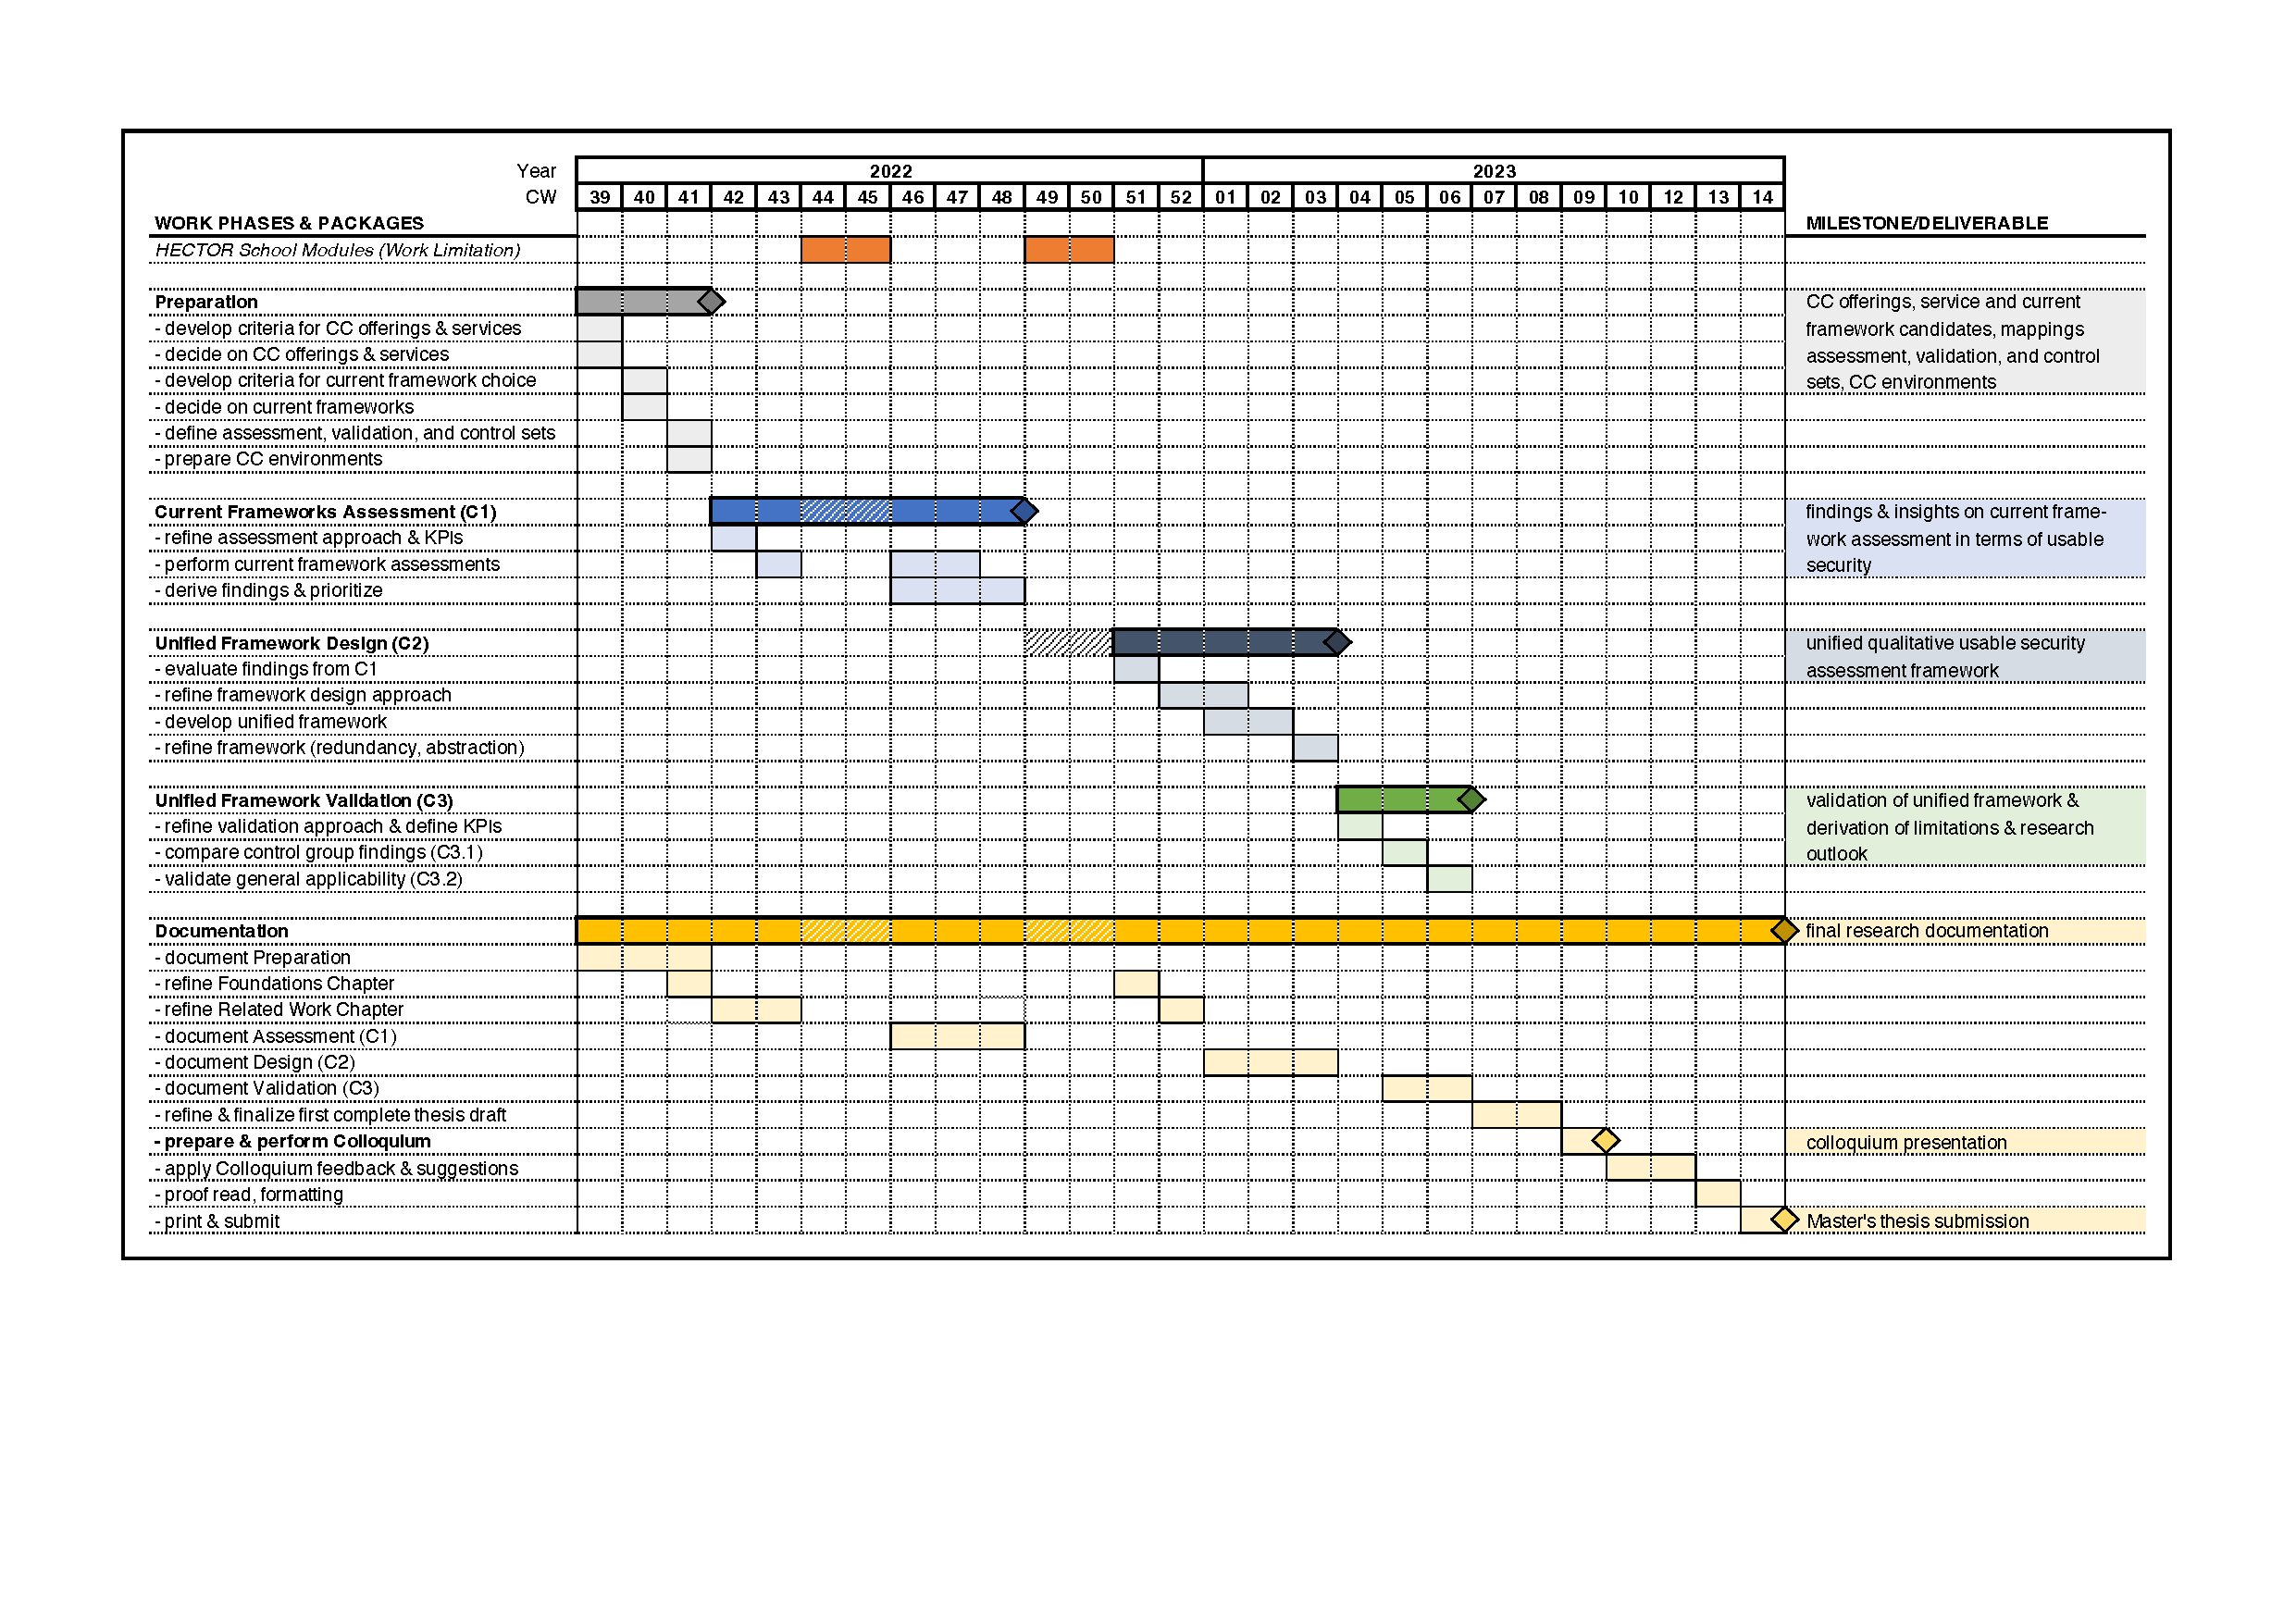
\includegraphics[angle=90,scale=0.58]{content/2-research-proposal/img/gantt.pdf}
		\vfill
	\end{center}
	\newpage